        %auto-ignore
\section{Additional Experiments}\label{sec:additional_exps}

\subsection{Failure of Standard Parametrization at Large Depths}

\begin{figure}[h]
    \centering
    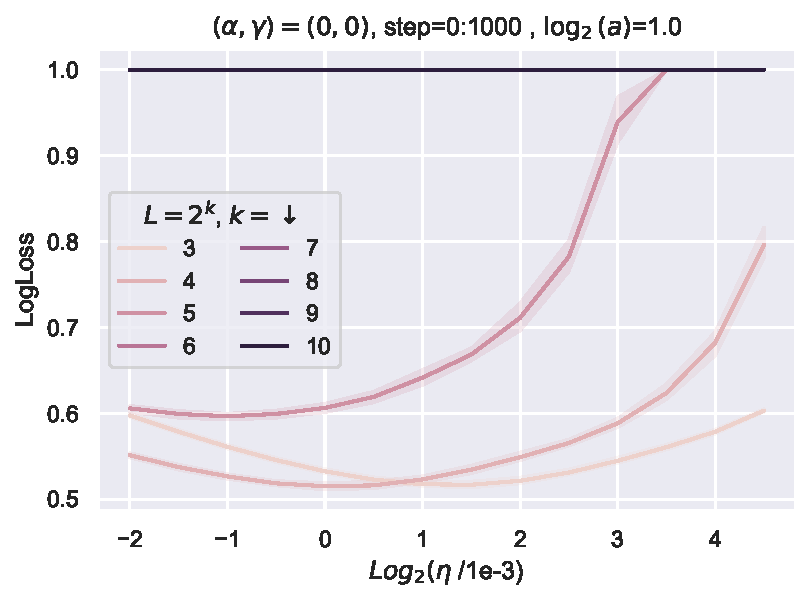
\includegraphics[width=0.45\linewidth]{fig/sp_0.pdf}
    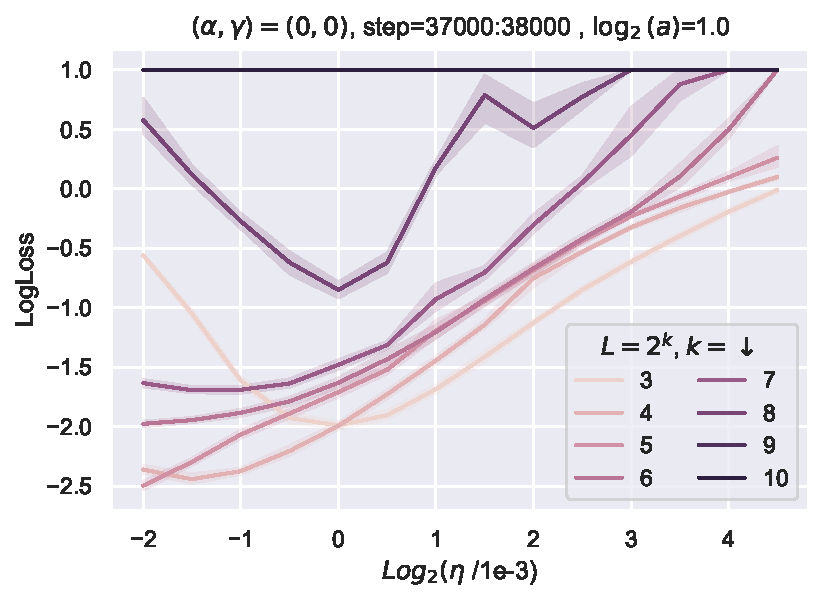
\includegraphics[width=0.45\linewidth]{fig/sp_37000.pdf}
    \caption{Training with Standard Parametrization fails at large depth due to numerical issues.}
    \label{fig:sp_failure}
\end{figure}

\subsection{Experiments with Block Depth 2}
Currently, our theory covers resnets with block depth 1, and our experiments confirm the theoretical findings. We conducted similar experiments for clock depth 2 (i.e. the residual block consists of 2 fully connected layers) to see whether the learning rate transfers with Depth-$\mu$P. The results are reported in \Cref{fig:bd2}. The results show a significant shift in the learning rate which might indicate that as block depth increases, adjustments are needed to stabilize hyperparameters with depth.

\begin{figure}
    \centering
    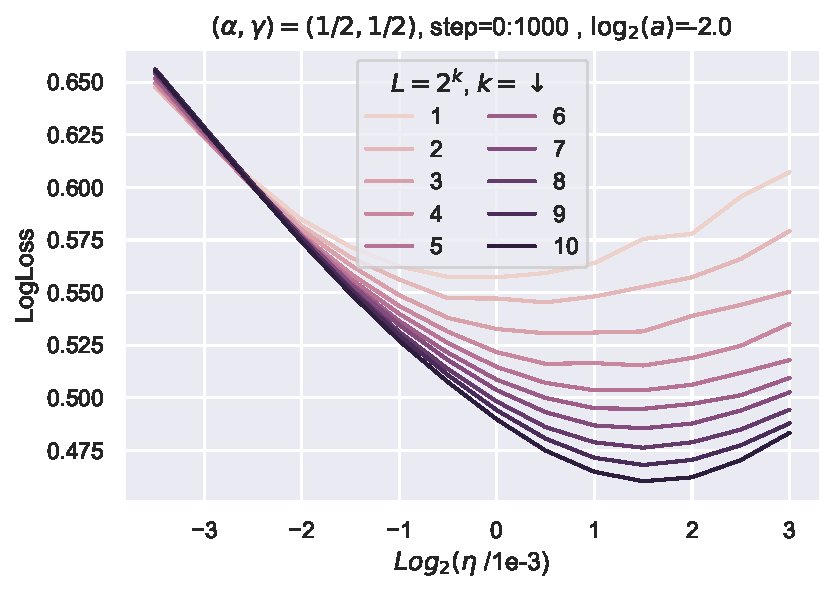
\includegraphics[width=0.45\linewidth]{fig/bd2_mup_0.pdf}
    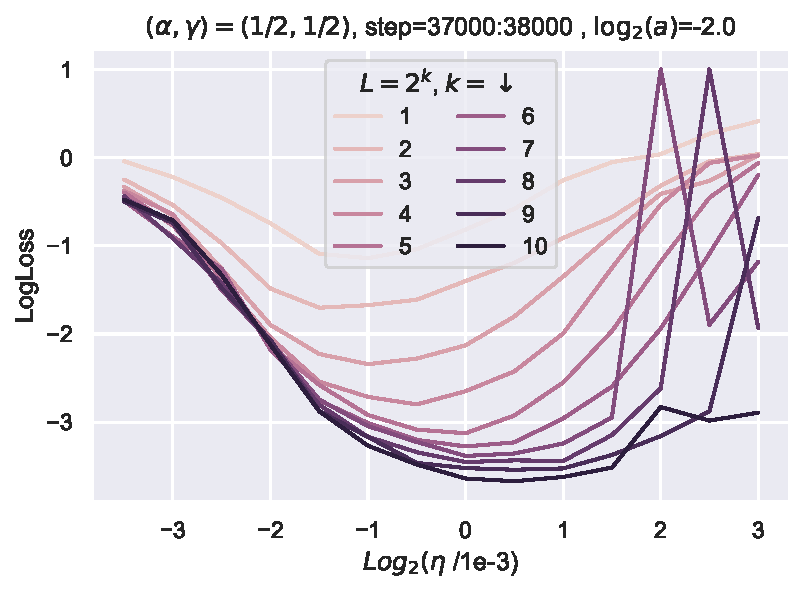
\includegraphics[width=0.45\linewidth]{fig/bd2_mup_37000.pdf}
    \caption{Same setup as \Cref{fig:lr_transfer}, with block depth 2 instead.}
    \label{fig:bd2}
\end{figure}

\subsection{Other experiments}

\begin{figure}[h]
    \centering
    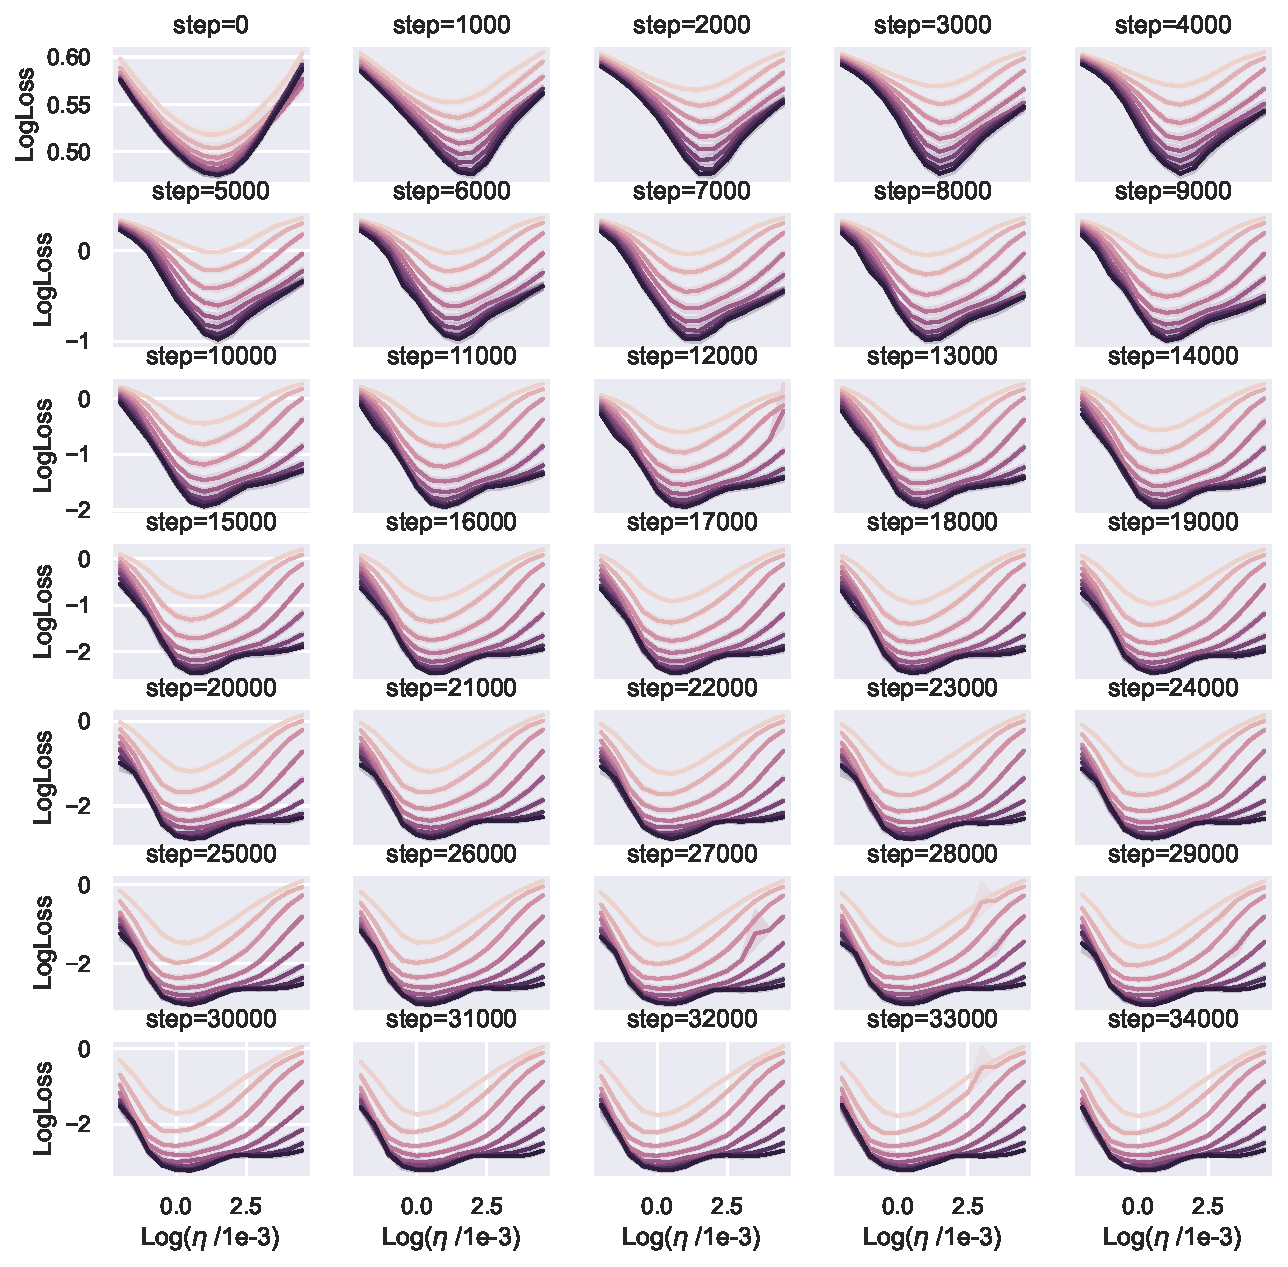
\includegraphics[width=\linewidth]{fig/mup_all_steps_Loss_VS_lr.pdf}
    \caption{Same as \cref{fig:lr_transfer} (\textbf{Up}, Depth-$\mu$P) with multiple time slices.}
    \label{fig:lr_transfer_all_mup}
\end{figure}

\begin{figure}[h]
    \centering
    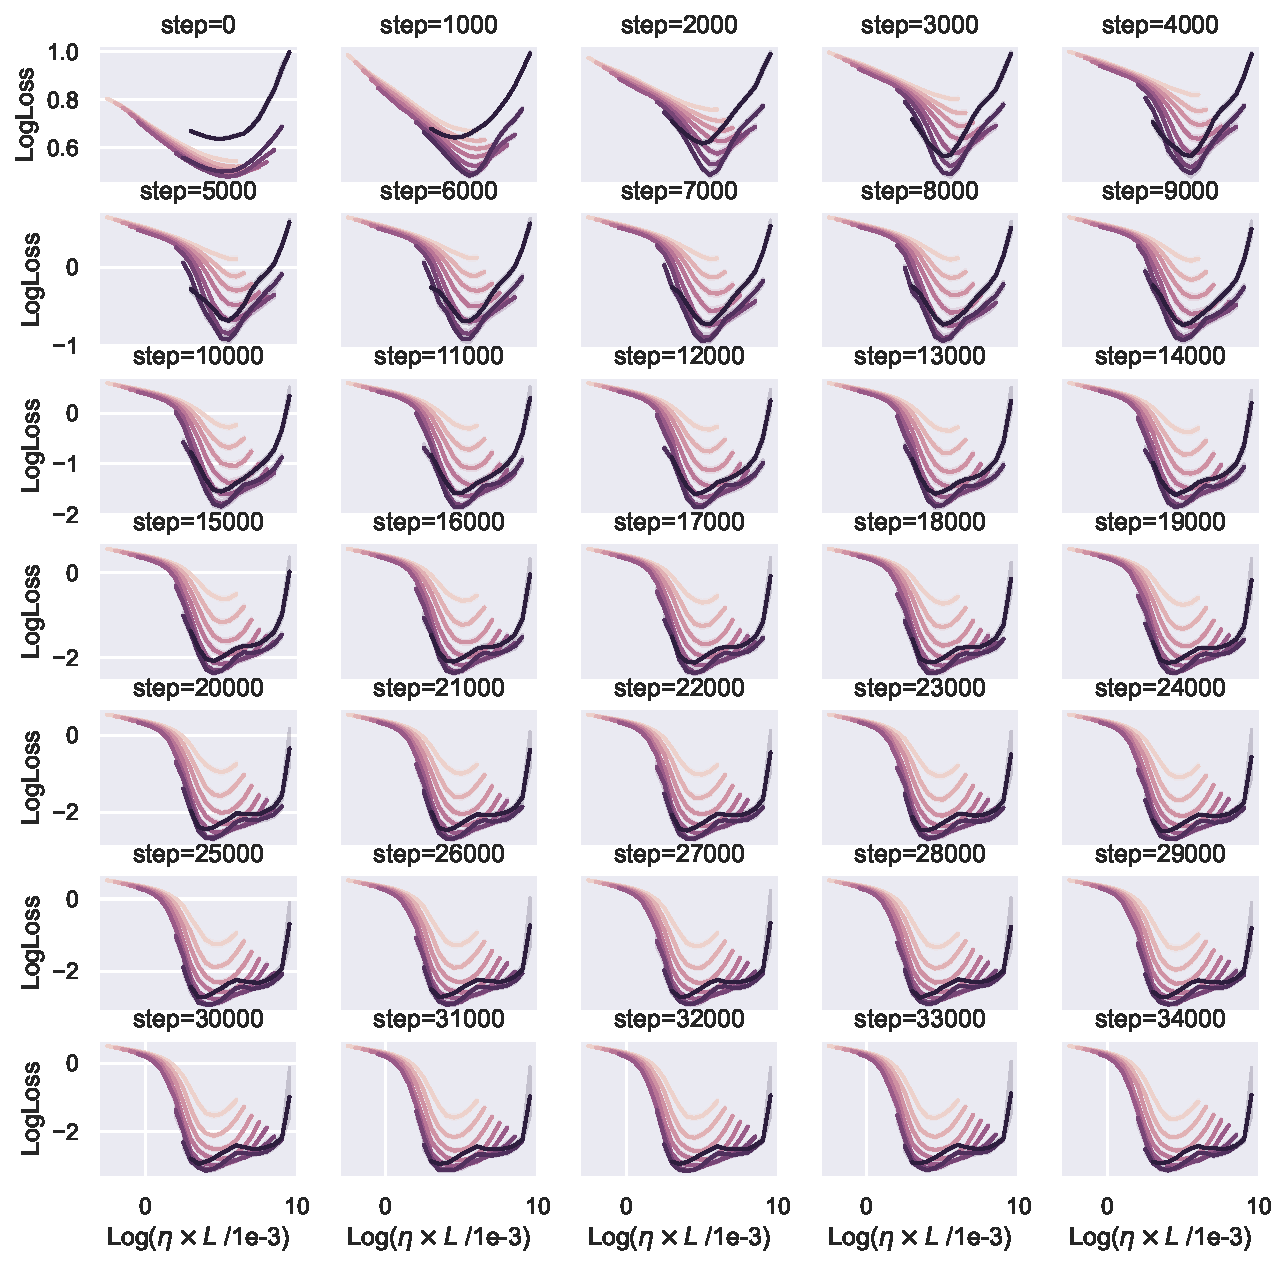
\includegraphics[width=\linewidth]{fig/sp_normalized_all_steps_Loss_VS_lr.pdf}
    \caption{Same as \cref{fig:lr_transfer} (\textbf{Middle}, Standard Parametrization with $\gamma = 1$) with multiple time slices.}
    \label{fig:lr_transfer_all_normalized_sp}
\end{figure}

\begin{figure}[h]
    \centering
    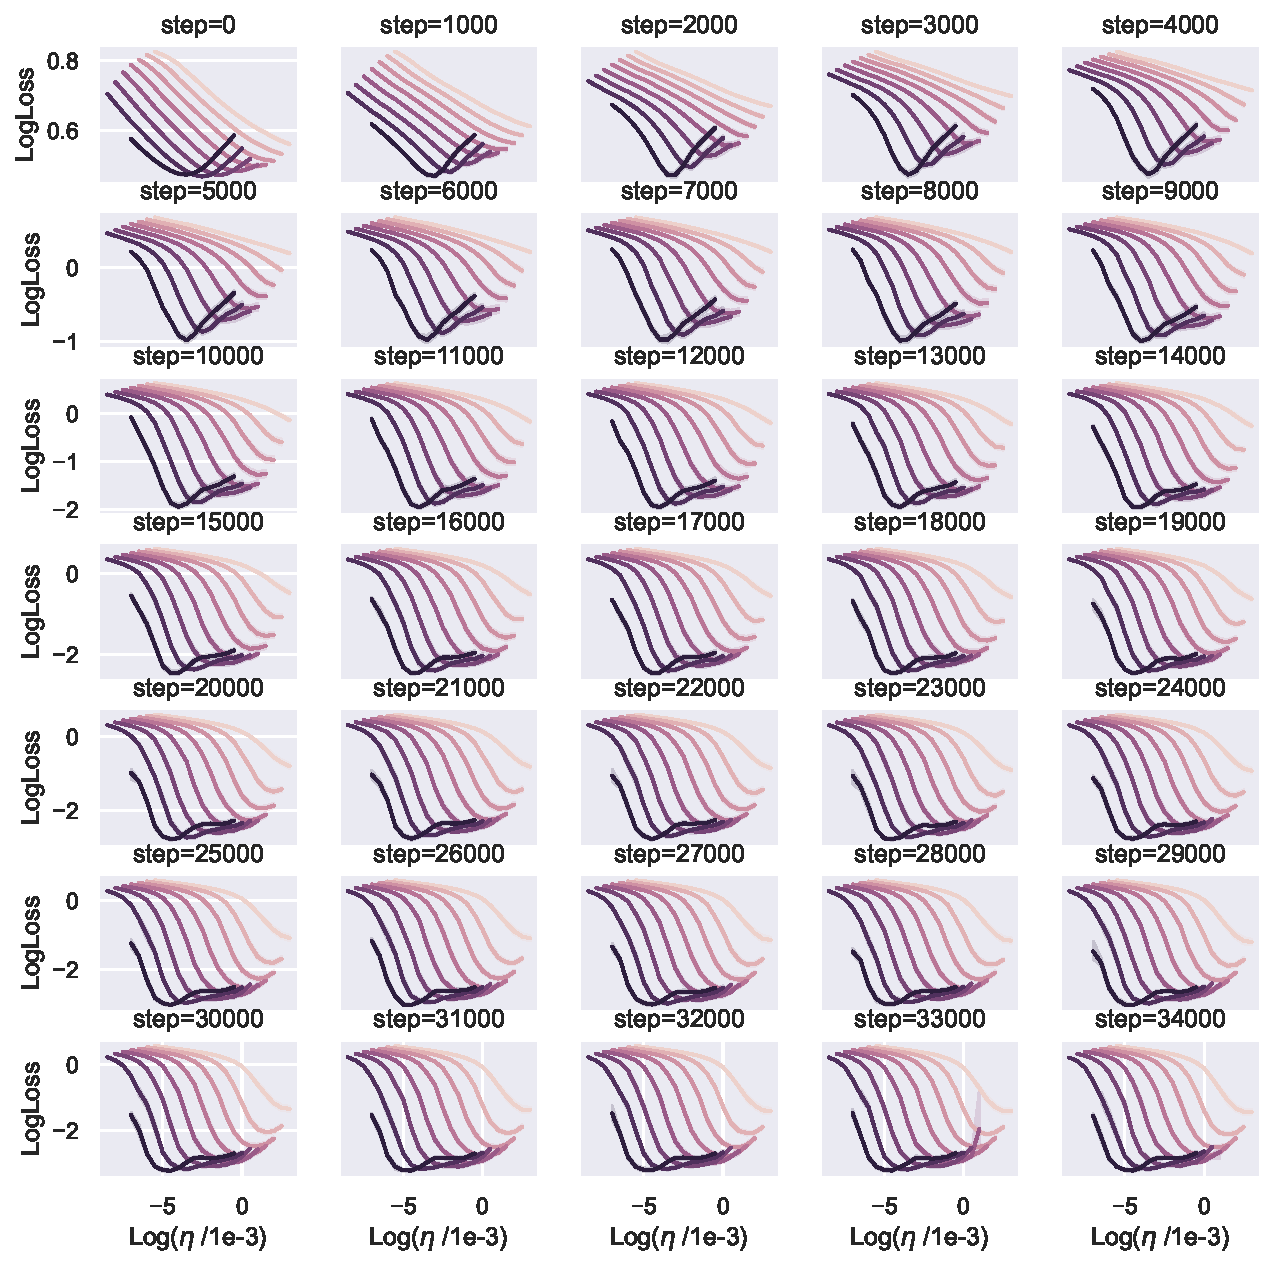
\includegraphics[width=\linewidth]{fig/sp_all_steps_Loss_VS_lr.pdf}
    \caption{Same as \cref{fig:lr_transfer} (\textbf{Bottom}, Standard Parametrization with no scaling, $\alpha=0, \gamma=0$) with multiple time slices.}
    \label{fig:lr_transfer_all_sp}
\end{figure}

\begin{figure}
    \centering
    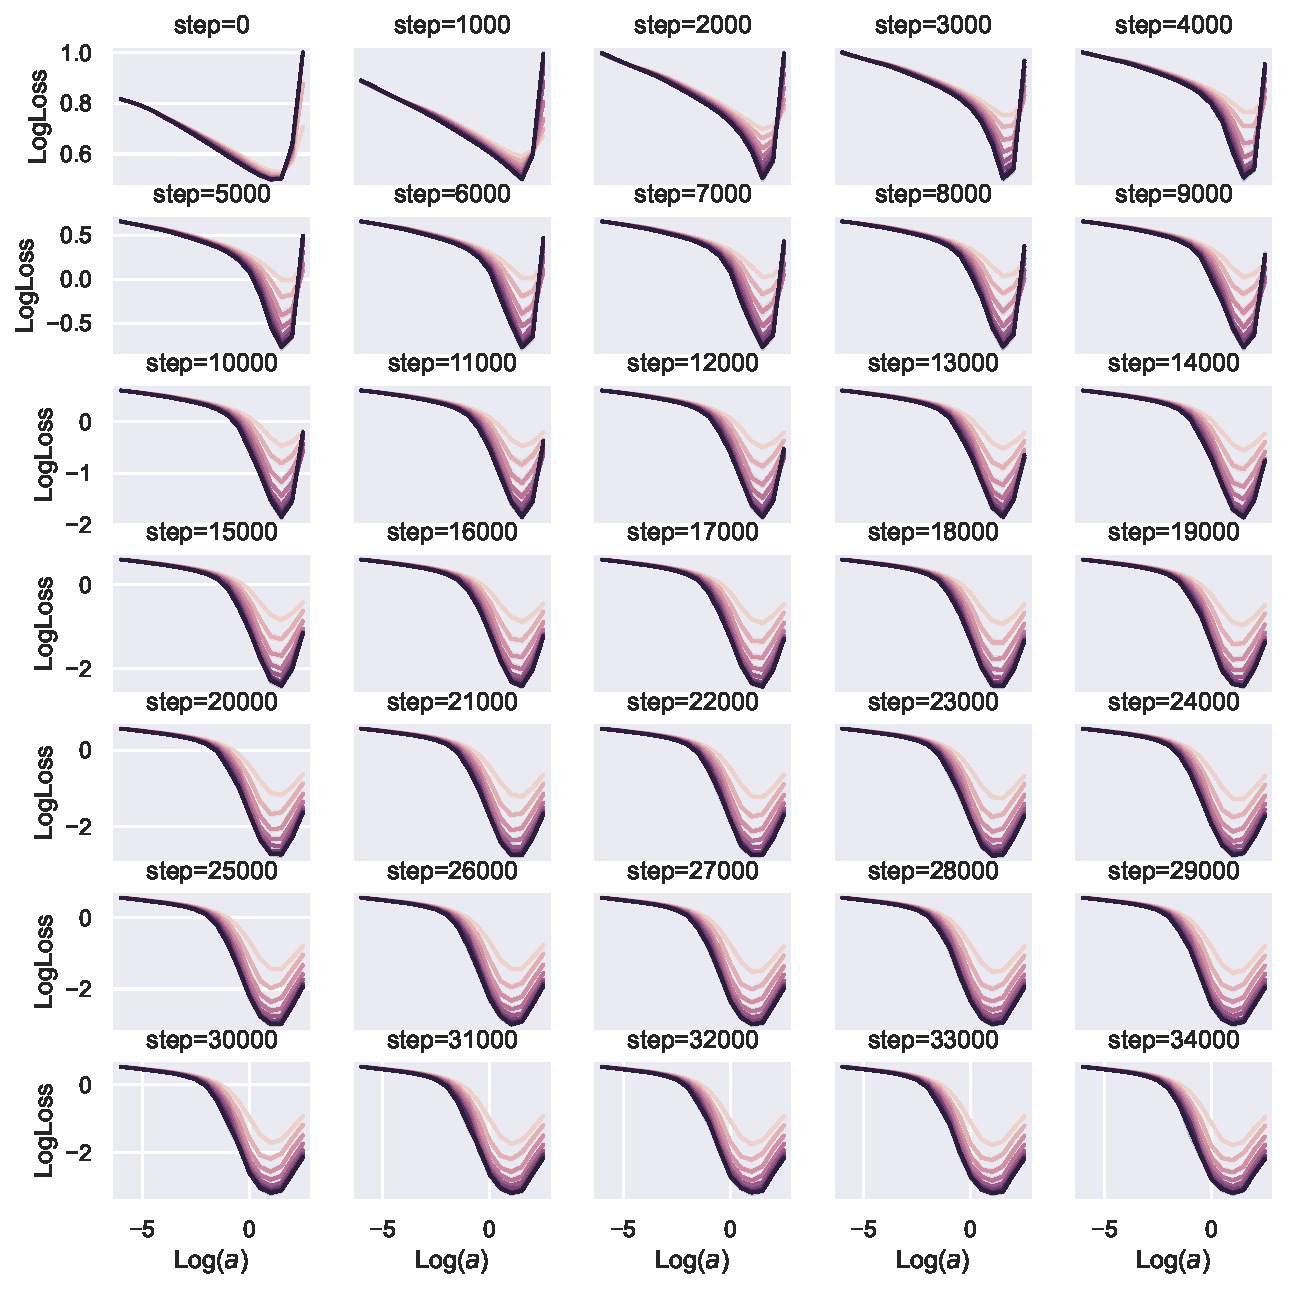
\includegraphics[width=\linewidth]{fig/mup_all_steps_Loss_VS_a.pdf}
    \caption{Same as \cref{fig:blockmult_transfer} with multiple time slices.}
    \label{fig:blockmult_transfer_all}
\end{figure}